% Dieses Dokuments muss mit XeLaTeX übersetzt werden!

% Wichtige Warnungen zur Nutzung von LaTeX
% Achtung: Muss in der ersten Zeile NOCH VOR \documentclass stehen!
% Quelle: http://www.howtotex.com/packages/9-essential-latex-packages-everyone-should-use/
\RequirePackage[l2tabu,orthodox]{nag}

\documentclass[12pt,listtotoc]{scrartcl}

% Für Schriftarten benötigt
% Löst fontenc bzw. inputenc unter XeLaTex und LuaTeX ab
%\usepackage{fontspec}
% Ersatz für babel unter XeLaTeX und LuaTeX (benötigt fontspec)
%\usepackage{polyglossia}
% Achtung: Möglichst früh aufrufen, damit Pakete übersetzt werden!
%\setmainlanguage[spelling=new,babelshorthands=true]{UKenglish}

% Schriftart setzen
%\setmainfont[Path=./fonts/,UprightFont=*-Regular,BoldFont=*-Bold]{SourceSerifPro}

% Pakete für Farbnamen und farbige Tabellen
\usepackage[table]{xcolor}

\usepackage{titlesec}

% Zum Einbinden von Grafiken
\usepackage{wrapfig}
\usepackage{graphicx}
\graphicspath{{images/}} % Pfad in geschweiften Klammern!

% Einrückung und Abstand von Absätzen
\usepackage{parskip}

% Klickbare URL
\usepackage[hidelinks]{hyperref}

% Shortcuts, Menüelemente und Pfade schöner formatieren
\usepackage{menukeys}

% Mehrere Zeilen in einer Tabelle in eine Zelle integrieren
\usepackage{multirow}

% Bessere Tabellen, v.a. Zeilenumbruch
\usepackage{ltablex}

% Bessere Kontrolle über Aufzählungen (z.B. Abstände)
\usepackage{enumitem}

% Für mathematische Umgebung, Zeichen etc.
\usepackage{amsmath}

% Schönere Tabellen
\usepackage{booktabs}

\usepackage{amssymb}

\setcounter{secnumdepth}{4}

\titleformat{\paragraph}
{\normalfont\normalsize\bfseries}{\theparagraph}{1em}{}
\titlespacing*{\paragraph}
{0pt}{3.25ex plus 1ex minus .2ex}{1.5ex plus .2ex}

%
%\bibdata{references/references}

\begin{document}
	
	\pagenumbering{roman}
	\begin{titlepage}
\begin{center}
\hbox{}
\vskip 3cm
\textsf{\scriptsize{Otto-Friedrich-Universität Bamberg}}\\
\vskip 5mm
\textsf{\footnotesize{Smart Environments und Kognitive Systeme}}
\vskip 3mm

\vspace{3mm}
\begin{center}
	
\includegraphics[width=25mm]{uniba-logo}
\end{center}
\vspace{3mm}
\vskip 8mm
\textsf{{\textbf{SME-Projekt-B:\\ AI-Birds}}}\\
\vskip 16mm
\textsf{\normalsize{Topic:}}\\
\vskip 8mm
\textsf{\Large{Meta}}\\
\vskip 40mm
\end{center}
\textsf{\normalsize{Autoren: Anne Schwarz, Susanna Cao}}\\
\textsf{\normalsize{Betreuer/-innen: Prof. Dr. Diedrich Wolter, Prof. Dr. Ute Schmid}}\\
\textsf{\normalsize{Bamberg, Sommersemester 2017}}\\
\vfill
\end{titlepage}


	\tableofcontents
	
	\pagebreak
	
	\listoffigures
	\pagebreak
	\pagenumbering{arabic}

	\section{Abstract}
Dieser Bericht stellt die Arbeit des Meta-Teams des Projekts SME-Projekt-B im Sommersemester 2017 vor. Begleitet wurde dies durch Prof. Dr. Diedrich Wolter sowie Prof. Dr. Ute Schmid. Ziel des Projekts ist die Entwicklung eines intelligenten Agenten, der am Wettbewerb ``Angry Birds AI Competition''\footnote{\url{https://aibirds.org/} (zuletzt abgerufen: 02.09.2017)} teilnimmt. \\
Das erste Kapitel gibt eine Einführung in das Thema und beschreibt die Problemstellung. Au\ss erdem wird darauf eingegangen, warum es von gro\ss er Bedeutung ist, genau für Angry Birds einen intelligenten Agenten zu entwickeln. \\
Das darauffolgende Kapitel umfasst zuerst das Thema, warum vor allem Angry Birds eine Herausforderung im Bereich der künstlichen Intelligenz darstellt. Danach folgt ein Überblick über den IJCAI 2017 Angry Birds AI Wettbewerb und es werden auf die Aufgaben des Meta-Teams eingegangen. Dabei wird auch eine grobe Beschreibung des Gesamtverlaufs des Agenten und seine einzelnen Komponenten neben dem Meta-Bereich gegeben. \\
Anschließend werden die wichtigsten Arbeitsbereiche der Meta-Gruppe und ihren Arbeitsverlauf im Detail vorgestellt.
Zum Schluss erfolgt ein Vergleich mit dem Agenten des letzten Jahres, wobei zusätzlich Vorschläge für einen besseren Agenten aufgeführt werden.

	\section{Einführung}
Angry Birds gilt als eines der beliebtesten und bekanntesten physik-basierten Simulationsspiele (engl. physics-based simulation game (PBSG)). Seit 2009 hat das Spiel über 200 Millionen Spieler weltweit angezogen. Das liegt u.a. daran, dass das Spielprinzip leicht zu verstehen und die Spielmechanik leicht erlernbar sind. Das Ziel von Angry Birds ist es alle Schweine und so viele Hindernisse wie möglich mit einer begrenzten Anzahl an Vögeln zu zerstören. Dazu werden diese mit Hilfe einer Schleuder auf eine Struktur geschossen, die sehr kompliziert sein kann und aus einer Reihe von verschiedenen Objekten mit unterschiedlichen Eigenschaften besteht. Wie in Abb. 1 ersichtlich gibt es unter anderem Bausteine aus Holz, Eis und Stein. Außerdem gibt es auch unterschiedliche Vögel, die jeweils spezifische Eigenschaften besitzen. So kann der gelbe Vogel z.B. effektiv Holz zerstören oder der schwarze Vogel Stein.

\begin{figure} [h]
\begin{center}
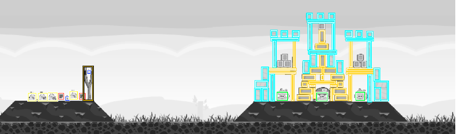
\includegraphics[width=150mm]{level.png}
\caption{Das Bild zeigt ein Level aus Angry Birds mit einer komplizierten Struktur, die aus verschiedenen Objekten mit unterschiedlichen Eigenschaften besteht. Hier dargestellt durch Bounding-Boxen.}
\end{center}
\end{figure}

Aus Sicht von Künstlicher Intelligenz vereint das Spiel Aspekte aus den Bereichen Computer Vision, Maschinelles Lernen, Wissensrepräsentation, Planen, Heuristische Suche und Schlussfolgern unter Unsicherheit. Einen intelligenten Agenten für dieses Spiel zu entwickeln, der besser sein soll als menschliche Spieler, ist genau deshalb für die Forschung von großer Bedeutung und stellt das Team vor schwierige Herausforderungen.
	\section{Hintergrund und Verwandte Arbeiten}

\subsection{Angry Birds als Herausforderung im Bereich Künstliche Intelligenz}
In physikbasierten Simulationsspielen wie Angry Birds ist die gesamte Spielwelt typischerweise parametrisiert. So sind beispielsweise alle physischen Parameter, wie die Masse, die Reibung, die Dichte von Objekten und die Gravität sowie alle Objekttypen und deren Eigenschaften und Lage intern bekannt. Jede gewählte Aktion kann deshalb mit einem zugrundeliegenden Physik-Simulator sehr realgetreu nachgebildet werden. Einfache Aktionen können wie folgt beschrieben werden: der Spieler kann erstens entscheiden an welchem Punkt <x,y> der Vogel aus der Schleuder gelassen werden soll und zweitens wann während des Flugs die Superkraft des Vogels aktiviert werden soll. In der Praxis ergibt dies eine sehr große Anzahl an möglichen Aktionen. Während des Spielens gilt ein Level immer dann als gelöst, wenn eine Reihe von Aktionen zu einem Spielstand führt, der bestimmte Siegbedingungen erfüllt.\\
Aus dem einfachen Spiel und den einfachen Aktionen resultiert, dass auch kleine Kinder das Spiel schon erfolgreich durchspielen können. Die Herausforderung des Wettbewerbs besteht also darin einen intelligenten Agenten zu bauen, der neue Level genauso gut oder sogar erfolgreicher spielen kann als die besten menschlichen Spieler. Im Vergleich zu scheinbar harten Spielen wie z.B. Schach klingt dies nach einer relativ einfachen Aufgabe, allerdings müssen einige Herausforderungen gemeistert werden. Unter der Annahme, dass alle Parameter der Spielwelt bekannt und parametrisiert sind, könnten Aktionen und deren Folgeaktionen solange simulieret werden bis der Siegzustand erreicht ist. Wenn die Handlungen dann noch intelligent ausgewählt werden, kann dies zu einer erfolgreichen Lösungsstrategie führen.\\
Hier liegt aber das Hauptproblem physikbasierter Simulationsspiele: das Ergebnis von Aktionen ist immer erst dann bekannt, wenn diese simuliert wird, was wiederum bedeutet, dass auch alle dafür benötigten Parameter bekannt sein müssen. Es liegt also eine andere Grundlage vor als bei Spielen wie Schach, in denen die Ergebnisse jeder Aktion schon im Voraus bekannt sind. Hinzu kommt, dass sich die Spielwelt nach jedem Schuss enorm verändert. Dies erfordert also präzise Vorhersagen oder Annäherungen an die resultierenden Konsequenten, um eine Strategie aus Aktionen entwickeln zu können. Die Kombination aus einem potentiell unendlichen Aktionsraum und dem möglichen Mangel an Informationen über alle Parameter stellt hinsichtlich des Treffens von Vorhersagen eine der größten Herausforderungen dar. Für den Menschen eine relativ einfache Aufgabe, allerdings ist das Kombinieren in unbekannten Umgebungen noch immer eine Forschungsfrage.\\
Die Forschung an physikbasierten Simulationsspielen wie Angry Birds ist deshalb so wichtig, weil die gleichen Probleme auch noch für AI-Systeme gelöst werden müssen, damit diese erfolgreich mit der physischen Welt interagieren können. Während Menschen diese Fähigkeit einfach haben und ständig einsetzen, ist aus Sicht von AI noch nicht das ganze Potential ausgeschöpft. Der IJCAI 2017 Angry Birds AI Wettbewerb bietet dazu eine geeignete Plattform an, um diese Herausforderungen und neuen Fähigkeiten in einer vereinfachten und kontrollierten Umgebung zu testen und zu entwickeln.

\subsection{Verwandte Arbeiten}
2013 veröffentlichte [Calimeri et al., 2013] den Artikel "AngryHEX: an Artificial Player for Angry Birds Based on Declarative Knowledge Bases". Diese Arbeit präsentiert ein gemeinsames Projekt der Universität von Kalabrien (UniCal) und der TU Wien, mit dem Ziel, einen intelligenten Agenten zu entwickeln, der am 2013 Angry Birds AI Wettbewerb teilnimmt. AngryHEX, so die Autoren, basiert auf einer Programmierung mit Hilfe von ASP (Answer Set Programming). Die grundlegende Spielsoftware, die von den Veranstaltern zur Verfügung gestellt wird, wurde ebenfalls verwendet. Diese wurde allerdings noch durch eine Erweiterung modifiziert, die Informationen über die aktuelle Szene in logische Behauptungen kodiert.\\
{[Ferreira et al., 2013]} beschreibt die Aufgabe des Projekts wie folgt. Laut den Autoren ist das Ziel einen autonomen Agenten zu entwickeln, der in der Lage ist, ohne menschliches Eingreifen [Angry Birds] zu spielen. Dabei ist dieser in der Lage ist seine Umgebung zu betrachten und mit einzubeziehen. Außerdem ist der Agent in der das beste Objekt als Ziel auszuwählen. Der Artikel beschreibt weiterhin die Entwicklung eines intelligenten Agenten namens FEI2, der für einen Wettbewerb 2012 entwickelt wurde. Der Schwerpunkt, so [Ferreira et al., 2013] weiter lag dabei auf der Auswahl des bestmöglichen Ziels. Zudem wurden für die Entwicklung drei Konzepte kombiniert. Einmal lag die Konzentration auf der räumlichen Darstellung der einzelnen Objekte, weil die Positionen der Objekte und die Lagebeziehungen derer untereinander wichtig seien. Die Autoren schreiben weiter: "The second concept is that of Utility Function, which allows the agent to represent preferences for the options that are given to it". Das zweite Konzept gibt dem Agenten also die Funktion Präferenzen für ein Zielobjekt abzugeben, dies ist wichtig bei der Entscheidungsfindung. Schließlich wurde als letztes Konzept Schlussfolgern unter Unsicherheit verwendet.\\
Mihai Polceanu und Cedric Buche konzentrieren sich in ihrem Artikel auf einen bestimmten Bereich für die Ausarbeitung eines intelligenten Agenten. Sie schreiben über verschiedene Entscheidungsmechanismen. Dabei liegt der Fokus vor allem auf der Erwartungsfähigkeit des Menschen und seiner Fähigkeit sich anzupassen, während diese interagieren. Da dieser Bereich auch für den intelligenten Agenten erarbeitet und implementiert werden soll, ist auch dieser Artikel sehr hilfreich bei der Ausarbeitung.

\subsection{Der IJCAI 2017 Angry Birds AI Wettbewerb}
Im Zuge des Wettbewerbs sollen die Fähigkeiten des entwickelten intelligenten Agenten für Angry Birds getestet werden. Dazu werden von Seiten der Veranstalter eine Vielzahl von Level angeboten, um in einer vereinfachten und kontrollierten Umgebung die Enticklung und Erprobung des Agenten voranzutreiben. Langfristig gesehen, soll der Wettbewerb beim Aufbau eines AI-Agenten unterstützen, der für ihn unbekannte Level besser spielen kann als die besten menschlichen Angry Birds Spieler.\\
Wie oben bereits beschrieben, ist dies ein sehr schwieriges Problem, da es erfordert, dass der Agent Handlungen vorhersagen kann, ohne aber die Spielwelt komplett zu kennen. Zusätzlich muss eine gute Handlungsauswahl implementiert werden.\\
Zu beachten ist, dass Level in beliebiger Reihenfolge gespielt und auch so oft wie nötig wiederholt werden können. Die Agenten werden danach anhand der insgesamt erreichten Punkte bewertet. Während des Wettbewerbs „Mensch gegen Maschine“ wird dann getestet, ob der Agent besser ist als menschliche Spieler. Folgende Probleme müssen dafür effizient gelöst werden:

\begin{itemize}
\item Erkennen und klassifizieren bekannter und unbekannter Objekte,
\item Erlernen von Eigenschaften der (unbekannten) Objekte und der Spielwelt,
\item Vorhersage des Handlungsergebnisses,
\item Auswahl guter Aktionen in vorgegebenen Situationen und
\item Planung einer erfolgreichen Aktionssequenz sowie
\item  der Reihenfolge in der Level gespielt werden sollen.
\end{itemize}

Gespielt wird die Google Chrome Version von Angry Birds, die unter chrome.angrybirds.com öffentlich zugänglich ist. Der zur Verfügung gestellte Wettkampfserver verbindet sich dadurch mit der zuvor eingerichteten Chrome Browser Erweiterung, durch die es möglich ist Screenshots des Spiels während der Laufzeit aufzunehmen. Außerdem können darüber auch die verschiedenen Aktionen per Mausklick ausgeführt werden. Teilnehmende Agenten, die sich auf verschiedenen Clients laufen müssen, können nur über ein festes Kommunikationsprotokoll mit dem Server interagieren. Dies ermöglicht dem Agenten das Anfordern von Screenshots, Aktionen und anderen Befehlen vom Server und das Ausführen dieser im Live-Spiel. U.a. kann auch der aktuelle Highscore jederzeit vom Server abgerufen werden. Den Agenten wird so die gleiche Information wie dem Menschen zur Verfügung gestellt. Die genaue Lage oder Parameter von Objekten bleiben allerdings trotzdem unbekannt.\\
Um das Problem zu vereinfachen und sich ganz auf die Entwicklung des Agenten zu konzentrieren, verwenden wir die von den Organisatoren zur Verfügung gestellte grundlegende Spielsoftware. Das Grundgerüst dieser Software besteht aus drei Komponenten:

\begin{itemize}
\item Computer-Vision-Komponente (engl.: computer vision component), die einen Ausschnitt des Videospiels analysieren kann und den Ort, die Kategorie und die Begrenzungsbox (Bounding Box) alles relevanten Objekte sowie den Spielstand indentifiziert
\item Trajektorien-Komponente (trajectory component), die Trajektorien von Vögeln berechnet und berechnet wohin man schießen muss, um ein bestimmtes Objekte oder einen bestimmten Ort zu treffen
\item -	Spielkomponente, die Aktionen ausführt und Screenshots erfasst.
\end{itemize}

\subsection{Meta-Strategie des Agenten "BamBird" 2017}
Für die Teilnahme am Wettbewerb hat sich das gesamte Projektteam in insgesamt vier Untergruppen geteilt. Jede Gruppe übernahm eine andere Aufgabe für die Entwicklung des Agenten. Die Aufteilung war wie folgt: Physiksimulation, Entwicklung neuer Schuss-Strategien, Anpassung des Schussmoduls und Meta-Strategie.\\
Das Zusammenspiel der Komponenten ist in folgendem Diagramm dargestellt:

\begin{figure} [h]
	\begin{center}
		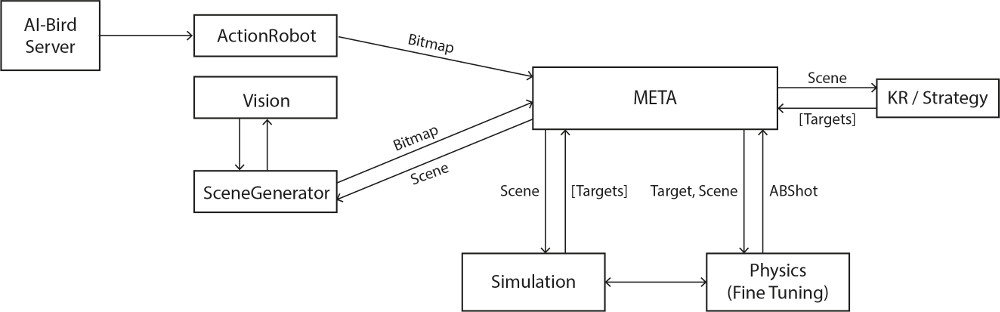
\includegraphics[width=1\textwidth]{ablaufdiagramm1}
		\caption{Wechselspiel der einzelnen Komponenten des Wettbewerbs.}
	\end{center}
\end{figure}

In diesem Bericht soll insbesondere auf die Arbeit des Meta-Teams eingegangen werden. Diese übergreift alle anderen Komponenten und führt diese zusammen, die Gruppe "Meta" ist also eine Art Schnittstelle für die anderen Gruppen.\\
Wir haben uns insbesondere folgenden Arbeitsfeldern angenommen. Als Erstes haben wir uns mit der Auswahl der verschiedenen Level während des Spiels beschäftigt. So nehmen wir Einfluss auf den Spielfluss und entscheiden in welcher Reihenfolge und wie oft die einzelnen Level gespielt werden sollen.
Eine weitere wichtige Aufgabe ist es, die richtigen Aktionen auszuwählen. Wir haben uns in dieser Hinsicht auf die Auswahl der Schüsse spezialisiert. Aus einer Liste, die wir von der Strategie-Gruppe erhalten, wählen wir, den als besten markierten Schuss aus. Zur Vorhersage einer guten Handlung haben wir uns des weiteren eine Form der Evaluation einzelner Schüsse überlegt, um besonders gute Schüsse zu kennzeichnen und diese in ähnlichen Situationen wieder anzuwenden.
Alle Informationen werden zu jedem einzelnen Schuss in einer Datenbank gespeichert, die wir implementiert haben.\\
Genaue Informationen über den Vorgang unserer Implementierung werden im folgenden Kapitel näher ausgeführt.
	\section{Key Results}
Dieser Abschnitt beschäftigt sich mit unserer Umsetzung der Aufgaben des Meta-Bereichs. Unser Ziel war es, nach jedem Durchlauf zu "lernen", indem man das vorherige Handeln speichert, evaluiert und dies beim wiederholten Durchlauf berücksichtigt.

\subsection{Level und Datenbank}

\subsubsection{Level}
Zur Speicherung der ausgeführten Aktionen wird eine Datenbank benötigt. Doch bevor man solch eine für die verschiedenen Level bauen kann, müssen die grundlegenden Informationen kompatibel sein: das Level selber. Unsere Java-Klasse \texttt{Level} befindet sich im Ordner \texttt{Meta}. Diese besteht aus der Level-ID, den geschätzten maximal zu erreichenden Punkten dieses Levels, den tatsächlich erreichten Punkten, der Anzahl der gespielten Durchgänge und einer Liste von ausgeführten Schüssen. Das Zusammenfassen der Schüsse erfolgt durch die selber errichtete Klasse \texttt{Triplet}, die sich auch im \texttt{Meta}-Ordner befindet. Hierbei wird neben dem eigentlichen Schuss (\texttt{shot}) zusätzlich noch das anvisierte Zielobjekt (\texttt{target}) und die allein aus diesem Schuss erreichten Punkte (\texttt{damagePoints}) gespeichert, welche später in der \texttt{ShotSelection} relevant sind. \\
Die Klasse an sich dient als Grundlage und enthält dementsprechend nur wenige Methoden, wobei einige bereits von der Gruppe aus dem letzten Jahr geschrieben wurden und wir nur noch unsere Änderungen anpassen mussten (siehe \texttt{addExecutedShot}) bzw. die Methoden verbessert haben (siehe \texttt{calculateEstimatedMaximalPoints}). 

\subsubsection{Datenbank}
Nach jedem Durchlauf eines Levels werden die oben genannten Informationen in ein \texttt{Level}-Objekt gespeichert. Jedes einzelne \texttt{Level}-Objekt wird dann in eine Datenbank hinzugefügt, welche unter \menu{ database > LevelStorage} zu finden ist. \\
Der Ordner \texttt{database} enthält eine weitere enum-Klasse \texttt{LevelState}, welche nur der Markierung der Level dient, weiter aber noch keine Verwendung findet. \\ 
Die \texttt{LevelStorage} besteht aus einer privaten Map, die die \texttt{Level} und den dazugehörigen \texttt{LevelState} beinhaltet. Zusätzlich enthält die Klasse eine öffentlichen Liste aus Integer, die in der gleichen Reihenfolge wie der Map die Level-IDs der gespielten Level speichert, sodass man von außen schnell auf die Information zugreifen kann, welche Level bereits gespielt wurden, sowie den Index der Level leichter abfragen kann. \\
Beim Speichern der Level muss darauf geachtet werden, dass man die Level nicht doppelt speichert im Falle eines wiederholten Versuchs. Daher prüfen wir in unserer öffentlichen Methode \texttt{addLeveltoStorage}, ob das übergebene Level bereits in der Datenbank erhalten ist. Falls es einen Eintrag mit dieser Level-ID gibt, wird die Hilfsmethode \texttt{updateLevelInfo} aufgerufen, welche nur die geänderten Einträge aktualisiert, anstatt einen komplett neuen Eintrag zu erstellen. \\
Die \texttt{LevelStorage} ist in der Evaluation von großer Bedeutung und wird in den Klassen der nachfolgenden Kapitel verwendet.

\subsection{Level Selection}
Die Klasse \texttt{LevelSelection}, die sich im Ordner \texttt{Meta} befindet, ist für die Levelauswahl zuständig. Sie hält die Information über die gesamte Anzahl der zu spielenden Level und über das Level, das gerade gespielt wird. Die Hauptmethode \texttt{selectNextLevel} beginnt mit einer zufällig ausgewählten Levelnummer und geht beim ersten Durchlauf alle Level der Reihenfolge nach durch. \\
Sobald alle Level einmal durchgespielt wurden, muss nun entschieden werden, welche Level in welcher Reihenfolge und wie oft wiederholt werden sollen. \\
Die Auswahl erfolgt nach einer simplen Wahrscheinlichkeitsberechnung für jedes einzelne Level, wobei das Level mit der höchsten Wahrscheinlichkeit ausgewählt wird: \\
$$ Probability = 1 - ( actualScore / maximalReachableScore ) $$
Wir richten uns also danach, wie viele Punkte wir von der maximal möglichen Punktzahl bereits abdecken konnten. \\
Eine Besonderheit gibt es für verlorene Level, welche als erste ausgewählt werden, denn ihre tatsächlich erbrachte Punktzahl beträgt 0 und sie haben somit eine Wahrscheinlichkeit von 1. Da man für jedes Level im Durchschnitt mindestens drei Minuten erhält \footnote{https://aibirds.org/angry-birds-ai-competition/competition-rules.html (zuletzt abgerufen: 05.09.2017)} und wir von einer Durchschnittsspieldauer von 1 - 1,5 Minuten pro Level ausgingen, entschieden wir uns, die verlorenen Level zunächst höchstens zweimal wiederholen zu lassen. Falls die Quote der verlorenen Level im Bezug auf die Gesamtanzahl der zu spielenden Level dann immer noch zu hoch ist, soll der Agent ein weiteres verlorenes Level auswählen. In unserem Fall haben wir die Grenze auf 15\% gesetzt, d.h. der Agent würde bei einer Gesamtanzahl von 21 Level einen erneuten Versuch starten, wenn mehr als 3 Level noch verloren sind. Falls dann immer noch nicht alle Level gewonnen wurden, sollen diese ignoriert werden. \\ 
Zur Veranschaulichung, wie der Algorithmus implementiert werden soll, dient der Pseudocode \ref{lvlSelec}. Hierbei haben wir einen boolean-Wert \texttt{ignoreLostLevels} integriert, der erst dann auf \textbf{true} gesetzt wird, wenn alle verlorenen Level zweimal wiederholt wurden und die Quote der verlorenen Level unter 15\% beträgt. Dieser Wert wird dann in der zweiten if-Schleife geprüft. \\
\begin{algorithm}[H]
  \begin{algorithmic}[1]
  	\State \textbf{boolean} \textit{ignoreLostLevels} = false
  	\\
  	\State \funccall{calculateProbabilities}() \Comment{calculates the probability for every level}
  	\\
  	\If{lost levels exist}
  		\If{all lost levels were repeated twice}
  		 	\If{Amount of lost levels > 15\% of total number of levels} 
  		 		\hspace{\algorithmicindent}  \Return \funccall{next lost level} \Comment{redo the lost levels one more time}
			\Else  
				\State \textit{ignoreLostLevels} = true
  		 	\EndIf
  		\Else
  			\Return \funccall{next lost level that has not been played twice yet}
  		\EndIf
  	\EndIf
  	\\
  	\If{no lost levels exist \textbf{or} \textit{ignoreLostLevels} == true}
		\Return level with the highest probability  	
  	\EndIf
  \end{algorithmic}
  \caption{Level selection after every level was played at least once \label{lvlSelec}}
\end{algorithm}

\subsection{Shot Selection}
Um bei wiederholten Versuchen von Level nicht ständig dieselben Schüsse zu nehmen und unsere Spieltaktik zu verbessern, kommt nun die Schussauswahl ins Spiel. Dafür bekommt unsere Klasse \texttt{ShotSelection}, die sich ebenfalls im \texttt{Meta}-Ordner befindet, von der Strategie-Gruppe für jeden Vogel eine Liste von Zielobjekten (\texttt{Targets}), auf die der Vogel schießen soll (siehe Methode \texttt{chooseShotWithOneList}). Eines davon wandeln wir dann in ein \texttt{Shot}-Objekt um und der Agent kann den Schuss dann im Spiel ausführen. Nachdem ein Schuss getätigt wurde, wird dieser dann für das entsprechende Level in eine Liste von Schüssen gespeichert (siehe Kapitel \textit{4.1.1 Level}).\\
Zu den jeweiligen \texttt{Targets} wird eine Konfidenz zwischen 0 und 1 mitübergeben, nach welcher der auszuführenden Schuss ausgewählt wird. 

\subsubsection{Verhindern von Wiederholen von Schüssen}
Hierbei besteht die Gefahr, dass immer derselbe Schuss genommen wird. Dies kann eintreten, wenn ein Schuss einer hohen Konfidenz zugeordnet wird, im echten Spiel jedoch wenig oder sogar keine Wirkung auf die Schweine und Gebäude hat. Da nach jedem Schuss neue Pläne in Bezug auf den jetzigen Stand der Umgebung generiert werden und sich die Szene nicht verändert, erhalten wir von der Strategie-Gruppe stets die gleiche Liste von Plänen. Würden wir also den Algorithmus ohne Einschränkung lassen, würde immer das Zielobjekt mit der höchsten Konfidenz ausgewählt werden, welches bei gleichen Szenen immer denselben Schuss entspricht. 
Somit haben wir einen Algorithmus integriert, der in Bezug auf die noch übrig gebliebenen Vögel entscheidet, ob der Schuss ein zweites Mal probiert werden soll, da es auch oft der Fall ist, dass der erste Schuss die Gebäude zum Wackeln gebracht hat und ein zweiter Schuss auf das gleiche Ziel ein guter Zug wäre. Dies lassen wir jedoch nur zu, wenn die Chance noch hoch genug ist, mit den restlichen Vögeln das Level trotz eines zweiten Fehlschusses noch gewinnen zu können. Dies wird in folgendem Pseudocode \ref{ShotSelec} veranschaulicht, wo wir uns nach des Gesamtzahl der Vögel richten: \\
\begin{algorithm}[H]
  \begin{algorithmic}[1]
  \If{shotCandidate.equals(previousShot)}
  	\If{(totalBirdAmount <= 3 \&\& executedShots >= 2) \textbf{or} \\ 
  	\hspace{\algorithmicindent} (totalBirdAmount > 3 \&\& previousPreviousShot.equals(previousShot))}
  	\\ \hspace{2.5em} \funccall{choose another shotCandidate}
  	\Else \\
  		\hspace{2.5em} \funccall{proceed with the current shotCandidate}
  	\EndIf
  \EndIf
  \end{algorithmic}
  \caption{Prevention of endless repetition in ShotSelection \label{ShotSelec}}
\end{algorithm}

\begin{table}[H]
\begin{itemize}
\item \textit{shotCandidate}: der zu prüfende Schuss, der ausgeführt werden soll 
\item \textit{previousShot}: der Schuss, der als letztes tatsächlich ausgeführt wurde
\item \textit{previousPreviousShot}: der Schuss, der vor dem zuletzt ausgeführten Schuss ausgeführt wurde
\end{itemize}
\end{table}

In unserem Algorithmus wird also nur derselbe Schuss noch einmal ausgeführt, wenn die Gesamtanzahl der Vögel über 3 beträgt und die zwei Schüsse davor nicht schon dieselben Schüsse waren, d.h. ein Schuss darf nicht mehr als einmal wiederholt werden. Im Falle von höchstens drei Vögel, wird ein anderer Schuss ausgewählt, wenn es sich gerade um den letzten Schuss handelt.

\subsubsection{Schussevaluation}
Falls das Level bereits gespielt wurde, überprüfen wir zunächst, ob der ausgewählte Schuss beim letzten Durchgang ebenfalls schon an dieser Stelle zum Einsatz kam und ob er ``gut'' oder ``schlecht'' war. Dementsprechend soll ein anderes Zielobjekt ausgewählt werden, wenn der Schuss als \textbf{BAD} markiert wurde. \\
Handelt es sich also bei dem momentanen \textit{shotCandidate}, um einen Schuss, der beim vorigen Durchgang bereits verwendet wurde, ruft die Methode \texttt{chooseShotWithOneList} die private Methode \texttt{evaluate} auf, in der die Schussevaluation erfolgt. Die Methode gibt dann ein enum -- \textbf{GOOD} oder \textbf{BAD} -- zurück. Bei der Evaluation werden zwei Aspekte berücksichtigt:
\begin{table}[H]
\begin{enumerate}
\item \textbf{Punktzahl von den einzelnen Schüssen} \\
Hierbei liegt der Fokus auf den Schaden, den der einzelne Schuss im Bezug auf den aktuellen Stand angerichtet hat. Wir rechnen nach jedem Schuss aus, wie viele Punkte noch maximal erreichbar sind, teilen dies dann durch die Anzahl der noch bestehenden Vögel, sodass wir einen Durchschnittswert erhalten, und geben zurück, wie viel der ausgeführte Schuss von diesem Durchschnittswert abdeckt. D.h. Falls man ein Level mit anfangs 5 Vögel hat und einer schon geschossen wurde, behandelt man das Level beim nächsten Schuss, wie wenn das Level nur 4 Vögel gehabt hätte und rechnet von dem Stand aus, wie viele Punkte noch maximal zu erreichen sind. Dieser Wert ist stets immer sehr hoch und eigentlich unmöglich zu erreichen, da bei der Berechnung des Maximalwerts davon ausgegangen wird, dass man mit einem einzigen Vogel alle Schweine und Konstruktionen, sowie die Bonuspunkte für übrig gebliebene Vögel erhält. Dementsprechend ist der errechnete Durchschnittswert für einen Schuss auch sehr hoch und je näher der Schuss diesem Wert kommt, desto besser wird der Schuss bewertet. Unserer Meinung nach, ist die erreichte Punktzahl eines Schusses ein ausschlaggebender Faktor, weshalb wir ihm eine Gewichtung von 0.7 in der Gesamtevaluation zuteilen (siehe \texttt{optimalShot}). \\
\item \textbf{Anzahl der Vögel bzw. Gesamtverlauf eines Levels} \\
Da es das Ziel von Angry Birds ist, mit wenig Vögeln alle Schweine zu vernichten und dabei so viel Schaden anzurichten wie möglich, muss auch die Gesamtbewertung, wie das Level beim letzten Durchgang ausging, in Betracht gezogen werden. Daher liegt der Fokus beim zweiten Aspekt auf der Anzahl der beim letzten Durchgang verwendeten Vögel. Wir rechnen dazu das Verhältnis aus, indem wir die tatsächlich verbrauchten Vögel durch die Gesamtanzahl teilen. Diesen Wert verrechnen wir dann mit einer Gewichtung von den restlichen 0.3 in die Gesamtevaluation mit ein (siehe \texttt{calculateRatioPoints}).
\end{enumerate}
\end{table}

Ist die Summe der beiden Werte dann kleiner als 0.45, markieren wir diesen Schuss als \textbf{BAD} und ein anderer zufälliger Schuss aus der übergebenen Liste wird ausgeführt.\\
Um auf diese Grenze zu kommen, haben wir einige Werte miteinander verglichen und uns selber überlegt, was wir für einen guten Schuss halten. Zuerst haben wir den ersten Punkt --Punktzahl der einzelnen Schüsse -- betrachtet: Wie hoch muss die Punktzahl sein, damit der Schuss als \textbf{GOOD} bewertet wird? Dazu haben wir uns die Werte aus Level 19 generieren lassen, welche in der Tabelle \ref{lvl19} aufgelistet sind.

\begin{figure}[H]
  \centering
    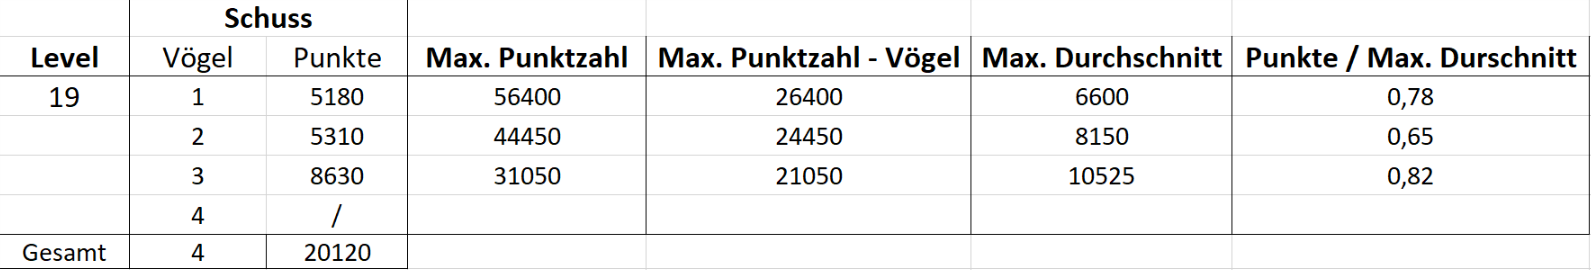
\includegraphics[width=1\textwidth]{Level19}
   \caption{Level 19}
   \label{lvl19}
\end{figure}

Da unserer Meinung nach alle Schüsse in diesem Level gut waren und wir den 2. Schuss noch an der Grenze zu gut sahen, stellten wir die Regel auf: der Schuss muss mind. 65\% von dem maximal zu erreichenden Durchschnittswert abdecken, um als guten Schuss zu gelten. \\
Ebenso sind wir auch mit dem zweiten Aspekt -- Anzahl der verwendeten Vögel -- vorgegangen und haben einige Szenarien durchgespielt, z.B. war es hervorragend, wenn der Agent höchstens 3 von 4, 3-4 von 5, 4 von 6, 5 von 7, 6 von 8 etc. Vögel verwendet hat. Mit diesen Vergleichen kamen wir dann auf einen Mittelwert von 75\%, d.h. wenn der Agent maximal 75\% der Verfügung gestellten Vögel verbraucht, gilt er als gut. Somit gilt: Je kleiner dieser Prozentsatz ist, desto besser ist die Gesamtbewertung. Daher muss mit dem Wert $Wert2 = 1 - ratio$ gerechnet werden. \\
Um diese beiden Werte dann in einem gemeinsamen Grenzwert zusammenfassen zu können, muss das Gesamtbild in Betracht gezogen werden. Abbildung \ref{evaluation} veranschaulicht alle Werte in einer Tabelle mit der Formel $0.7 * Wert1 + 0.3 * Wert2$, wobei $Wert1$ den verrechneten Wert der Punktzahl des einzelnen Schusses und $Wert2$ das Verhältnis für die Anzahl der Vögel darstellt:

\begin{figure}[H]
  \centering
    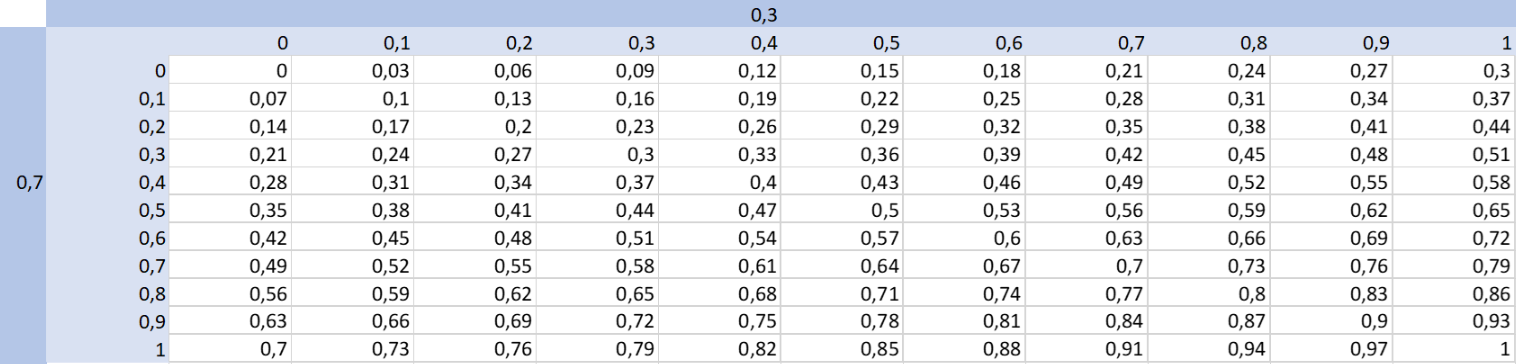
\includegraphics[width=1\textwidth]{EvaluationsWerte}
   \caption{Evaluationswerte}
   \label{evaluation}
\end{figure}

Unsere erste Bedingung ist, dass falls $Wert1 > 0.65$ die Gesamtbewertung gut ist, auch wenn alle Vögel verwendet wurden. Dadurch folgt: $0.7 * 0.65 + 0.3 * 0 = 0.455$. \\
Diese Grenze lässt sich auch gut auf andere Fälle anwenden, was auch anhand der Tabelle \ref{evaluation} zu sehen ist, z.B. um den betrachteten Schuss noch als \texttt{GOOD} zu markieren muss er mind. 60\% von der maximal zu erreichenden Durchschnittspunktzahl abdecken, wenn er 80\% aller Vögel verwendet hat -- $0.7 * 0.6 + 0.3 * 0.2 = 0.48$. Andernfalls gilt er als \texttt{BAD}. Im Kontrast, wenn der Agent beispielsweise bei dem Schuss nur 2 von 5 Vögeln benötigt hat, d.h. $Wert2 = 1 - 2/5 = 0.6$, muss die erreichte Punktzahl des Schusses nur 40\% betragen, um die Grenze zum guten Schuss zu überschreiten.

\subsection{Meta}
Das Zusammenspiel aller oben genannten Klassen findet in der \menu{ meta > Meta}-Klasse statt, welche von der Hauptinstanz \menu{ main > Bambird} aufgerufen wird. Diese Klasse stellt die Verbindung zum tatsächlichen Spiel und dem Server dar. \\
Ein Objekt der Klasse \texttt{Meta} wird genau einmal aufgerufen und entspricht der eigentlichen Main-Methode. Zur Veranschaulichung des Aufbaus dieser Klasse dient der Pseudocode \ref{meta}.

\begin{algorithm}[H]
  \begin{algorithmic}[1]
  \Loop
  	\If{GameState != Playing}
  		\State choose new Level
  	\EndIf
  	\State take a screenshot from the scene and analyse
  	\State generate plans
  	\State choose one plan to be executed as a shot
  	\State execute chosen shot
  	\State add shot to the shot-list of the current level
  	\If{GameState == WON or GameState == LOST} \\
  		\hspace{2.5em} add level to database
  	\EndIf
  \EndLoop
  \end{algorithmic}
  \caption{Meta \label{meta}}
\end{algorithm}

Die Schleife läuft ständig bis das Spiel zu Ende ist. Es wird ein Level ausgewählt und jeder ausgeführte Schuss wird in dem Level gespeichert und der nächste Schuss wird ausgeführt. Nach jedem vollendeten Level wird es dann in die Datenbank gespeichert und die Schleife beginnt von vorne, wobei es diesem Fall in die erste If-Schleife kommt und ein neues Level auswählt.
	\section{Konklusion}

\subsection{Wettbewerb}
Der Wettbewerb fand am 24.8.2017 statt, wobei wir dieses Jahr den Titel leider nicht verteidigen konnten. Das Problem lag daran, dass wir an einem Level hängen geblieben sind und uns das soviel Zeit gekostet hat, dass wir nicht mehr in der Lage waren dies aufzuholen. \footnote{\url{https://aibirds.org/angry-birds-ai-competition/competition-results.html} (zuletzt abgerufen: 13.09.2017)} Ob damit gemeint war, dass keine passende Strategie gefunden wurde oder ob es immer wieder das gleiche Level ausgewählt hat, konnten wir leider nicht in Erfahrung bringen.

\subsection{Vergleich zu letztem Jahr}
Der signifikanteste Unterschied zwischen unserer Vorgehensweise und der aus dem letzten Jahr ist die Verwendung der Datenbank. Während das Team 2016 keinen Speicher verwendet hat und ihre Taktik auf Zufall basierte, bauen unsere Ideen zur Verbesserung und zum Lernen der Spieltaktik auf der Level-Storage auf. Dementsprechend fehlte dem Team aus letztem Jahr auch eine Schussauswahl. \\
Am meisten ähnelt sich jedoch die Levelauswahl, wobei wir ihre Idee für die Grenze, die wir für die Anzahl an Wiederholungsversuchen zulassen, auch in unseren Gedankengängen in Betracht gezogen haben (siehe Kapitel 8.3 - \glqq A case study on the level selection functionality\grqq aus dem Projektbericht 2016). Wir haben ihre Ideen sozusagen erweitert.

\subsection{Verbesserungsmöglichkeiten}
\subsubsection{Datenbank}
Derzeit verwendet die \texttt{LevelStorage} eine Map und eine separate Liste, die die Level-IDs umfasst. Es wäre übersichtlicher eine einzige Liste oder Map zu haben und diese als Einheit zu verwenden. \\
Au\ss erdem könnte der Speicher erweitert werden. Was auf jeden Fall verbessert werden muss, ist dass es mehrere Listen bzw. eine gro\ss e Liste von allen Schüssen geben muss. In der jetzigen Implementierung wird die Schussliste eines Levels nach dem Wiederholen desselben Levels lediglich überschrieben, d.h. man verliert die Information der Schüsse aus dem ersten Durchgang. \\
Zusätzlich können noch andere Merkmale gespeichert werden, abhängig von den anderen Gruppen, z.B. Ergebnisse der Physiksimulation. Eine sinnvolle Idee wäre es auch, komplette Levelszenen zu speichern, also die Strukturen und ihre Reihenfolge, Anzahl der Vögel und Anzahl der Schweine. Somit können die einzelnen Level genauer analysiert und evaluiert werden.
\subsubsection{Levelauswahl}
Bei der Levelauswahl könnte man eine andere Formel finden, um die Wahrscheinlichkeit für ein Level zu berechnen, sowie andere Komponenten mit einbeziehen. Ebenfalls können andere Grenzen gesetzt werden, wie oft ein Level gespielt werden darf und die Reihenfolge nicht nur abhängig von der erreichten Punktzahl machen, sondern auch auf die verbliebene Zeit und das Ausma\ss  des Levelumfangs, sodass man ab einer bestimmten Zeit beispielsweise nur noch kleinere Level spielt, um noch so viele Level spielen zu können wie möglich.
\subsubsection{Schussauswahl und Evaluation}
Für die Schussauswahl könnte das Meta-Team, falls die Physiksimulation hinzukommt, eigene Konfidenzen für die übergebenen Pläne errechnen, anstatt sich allein auf das Strategie-Team zu verlassen.  \\
Derzeit erfolgt die Schussevaluation so, dass wir nur Schüsse vergleichen, die im selben Level an der gleichen Stelle ausgewählt werden und der erste Durchgang aller Level erfolgt somit ohne Evaluation. Man könnte einen Weg finden über die Level hinaus Schüsse zu vergleichen. Ein Ansatz wäre die Erweiterung der Datenbank um das Speichern von ganzen Welten. Dadurch können die Schüsse bereits beim ersten Durchgang verglichen werden, z.B. besitzt Level 1 eine ähnliche Struktur wie Level 4, könnte man sich den Schuss auf diese Struktur aus Level 1 zur Hilfe für Level 4 nehmen. 

\subsection{Fazit}
Alles in Einem sind wir der Meinung, dass der Agent trotz des Versagens im Wettbewerb gelungen ist und nach der Umstrukturierung eine gute Basis zu einem hervorragenden Agenten besitzt. Beim nächsten Mal kann der Fokus mehr auf maschinelles Lernen und tiefer gehende Aspekte eingegangen werden.
	%\section{References}


	\bibliography{references/references}
	\bibliographystyle{plain}
	
\end{document}
